\documentclass[tikz,12pt,border=2pt]{standalone}
\usepackage[T1]{fontenc}
\usepackage[scaled=0.92]{helvet}
\renewcommand{\familydefault}{\sfdefault}
\usetikzlibrary{calc,arrows.meta}
\definecolor{accent}{RGB}{31,84,140}
\definecolor{accentlight}{RGB}{200,214,232}
\begin{document}
\hyphenpenalty=10000\exhyphenpenalty=10000
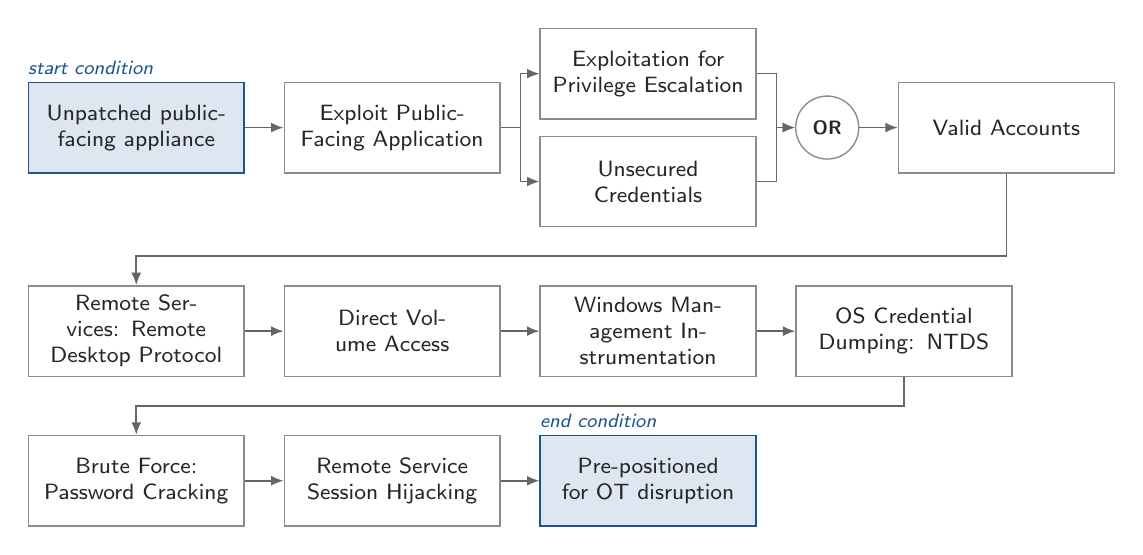
\begin{tikzpicture}[x=1cm,y=1cm,box/.style={draw=black!45,line width=0.5pt,fill=white,align=center,text width=2.530cm,minimum height=1.150cm,inner xsep=3pt,inner ysep=2pt,text=black!85,font=\fontsize{8pt}{9.44pt}\selectfont},cond/.style={box,draw=accent,fill=accentlight!60},op/.style={circle,fill=white,draw=black!45,line width=0.5pt,minimum size=0.800cm,inner sep=0pt,text=black!85,font=\fontsize{7.5pt}{8.85pt}\selectfont\bfseries},tag/.style={anchor=south west,inner sep=0pt,text=accent,font=\fontsize{7.5pt}{8.85pt}\selectfont\itshape},edge/.style={draw=black!60,line width=0.6pt,-{Latex[length=4.5pt,width=3.6pt]}}]
\node[cond] (n0) at (1.375,-1.260) {Unpatched public-facing appliance};
\node[tag] at ($(n0.north west)+(0,0.08)$) {start condition};
\node[box] (n1) at (4.625,-1.260) {Exploit Public-Facing Application};
\node[box] (n2) at (7.875,-0.575) {Exploitation for Privilege Escalation};
\node[box] (n3) at (7.875,-1.945) {Unsecured Credentials};
\node[op] (n4) at (10.150,-1.260) {OR};
\node[box] (n5) at (12.425,-1.260) {Valid Accounts};
\node[box] (n6) at (1.375,-3.845) {Remote Services: Remote Desktop Protocol};
\node[box] (n7) at (4.625,-3.845) {Direct Volume Access};
\node[box] (n8) at (7.875,-3.845) {Windows Management Instrumentation};
\node[box] (n9) at (11.125,-3.845) {OS Credential Dumping: NTDS};
\node[box] (n10) at (1.375,-5.745) {Brute Force: Password Cracking};
\node[box] (n11) at (4.625,-5.745) {Remote Service Session Hijacking};
\node[cond] (n12) at (7.875,-5.745) {Pre-positioned for OT disruption};
\node[tag] at ($(n12.north west)+(0,0.08)$) {end condition};
\draw[edge] (n0.east) -- ++(0.250,0) |- (n1.west);
\draw[edge] (n1.east) -- ++(0.250,0) |- (n2.west);
\draw[edge] (n1.east) -- ++(0.250,0) |- (n3.west);
\draw[edge] (n2.east) -- ++(0.250,0) |- (n4.west);
\draw[edge] (n3.east) -- ++(0.250,0) |- (n4.west);
\draw[edge] (n4.east) -- ++(0.250,0) |- (n5.west);
\draw[edge] (n5.south) -- (n5.south |- 0,-2.895) -| (n6.north);
\draw[edge] (n6.east) -- ++(0.250,0) |- (n7.west);
\draw[edge] (n7.east) -- ++(0.250,0) |- (n8.west);
\draw[edge] (n8.east) -- ++(0.250,0) |- (n9.west);
\draw[edge] (n9.south) -- (n9.south |- 0,-4.795) -| (n10.north);
\draw[edge] (n10.east) -- ++(0.250,0) |- (n11.west);
\draw[edge] (n11.east) -- ++(0.250,0) |- (n12.west);
\end{tikzpicture}
\end{document}
